
\documentclass{beamer}

%Style
\mode<presentation>
{
\usetheme{Frankfurt}

\setbeamercovered{transparent}
}

%Packages
\usepackage[english]{babel}
\usepackage[latin1]{inputenc} 

\usepackage{ae}

\usepackage[T1]{fontenc}

\usepackage{graphicx,wrapfig,lipsum}

\usepackage{listings}
\lstset{frame=shadowbox, rulesepcolor=\color{gray}, language=XML, basicstyle=\scriptsize}
%-----Title Page
\title{Web Services}

\subtitle{Web Services with AXIS}

\author{Javlon Eraliyev}

\date{Linz, Austria\\2013}

\subject{Practical Software Technology}

\pgfdeclareimage[height=0.7cm]{university-logo}{../pics/jku}
\logo{\pgfuseimage{university-logo}}

%\beamerdefaultoverlayspecification{<+->}

%-----Main
\begin{document}

%Title
\begin{frame}
\titlepage
\end{frame}

%TOfContents
\begin{frame}
\frametitle{Contents}
\tableofcontents
% You might wish to add the option [pausesections]
\end{frame}

\section{Web Services}

\subsection[Short First Subsection Name]{Concept }

\begin{frame}
\frametitle{Web Service}
\framesubtitle{is a method of communication between two electronic devices over the World Wide Web.}

\begin{figure}
\centering
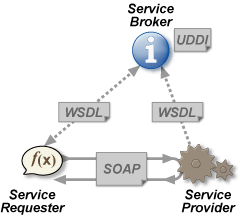
\includegraphics[scale=0.7]{../pics/Webservices.png}
\caption{Web services architecture}
\label{overflow}
\end{figure}
 
\end{frame}


\subsection[Short First Subsection Name]{SOAP} 

\begin{frame}
\frametitle{SOAP = XML + HTTP + Standarts}
\framesubtitle{Simple Object Access Protocol}
\begin{itemize}
  \item SOAP is a method of transferring messages, or small amounts of information, over the Internet.
  \item SOAP messages are formatted in XML and are typically sent using HTTP  
  \item For example, a user can send a SOAP message from a Windows machine to a Unix-based Web server without worrying about the message being altered
\end{itemize}
\end{frame}

\begin{frame}
\frametitle{Example: SOAP} 
\lstinputlisting{soap.xml}
\end{frame}


\subsection[Short First Subsection Name]{WSDL}

\begin{frame}
\frametitle{WSDL}
\framesubtitle{Web Services Description Language}
WSDL is an XML-based interface description language that is used 
for describing the functionality offered by a web service.

Describes:
\begin{itemize}
  \item How the service can be called 
  \item What parameters it expects
  \item What data structures it returns
\end{itemize}

\begin{figure}
\centering
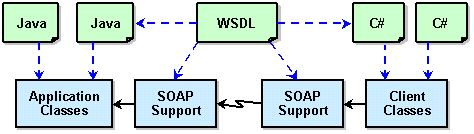
\includegraphics{../pics/wsdl.jpg}
\caption{How two different languages can deal}
\label{overflow}
\end{figure}

\end{frame}

\begin{frame}
\frametitle{Example: WSDL} 
\lstinputlisting{wsdl.xml}
\end{frame}


\subsection[Short First Subsection Name]{UDDI}

\begin{frame}
\frametitle{UDDI}
\framesubtitle{Universal Description Discovery and Integration = XML-based registry}
\begin{itemize}
  \item Provides a standardized method for publishing and discovering information about web services.  
  \item UDDI registries are used in an enterprise to share Web Services
\end{itemize}

\begin{figure}
\centering
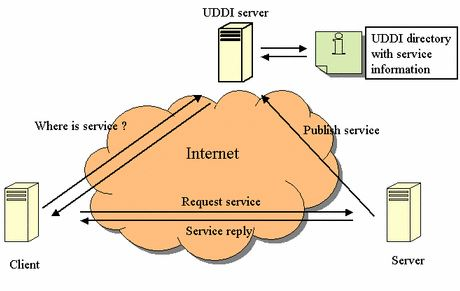
\includegraphics[height=130]{../pics/uddi.jpg}
\caption{Service lookup using UDDI}
\label{overflow}
\end{figure}

\end{frame}

\subsection[Short First Subsection Name]{Overview}

\begin{frame}
\frametitle{Overview}

\begin{wrapfigure}{r}{140}
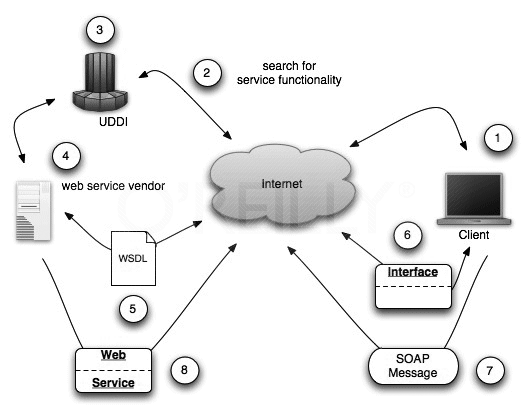
\includegraphics[width=170]{../pics/overview.png}
\label{overflow}
\end{wrapfigure}

{\scriptsize
[1]Seek out service;\newline
[2]Connect to the directory to discover a relevant service\newline 
[3]Determine the presence of a service;\newline 
[4]Check on availability and validity of vendor;\newline
[5]Vendor sends the client a WSDL;\newline
[6]Instance of the WS\newline
[7]SOAP requestes\newline
[8]Return values, responses
}

\end{frame}

\begin{frame}
\frametitle{Example: WSDL} 
\lstinputlisting{wsdl.xml}
\end{frame}



\section{Web Services with AXIS}

\begin{frame}
\frametitle{AXIS}
Axis is essentially a SOAP engine -- a framework for 
constructing SOAP processors such as clients, servers, 
gateways, etc. The current version of Axis is written in Java.

It also includes:
\begin{itemize}
  \item a simple stand-alone server
  \item a server which plugs into servlet engines such as Tomcat
  \item extensive support for the WSDL
  \item emitter tooling that generates Java classes from WSDL
  \item a tool for monitoring TCP/IP packets
\end{itemize}
\end{frame}

\subsection[Short First Subsection Name]{Installation and Usage}

\begin{frame}
\frametitle{Installation and Usage}
\framesubtitle{Apache Axis2 Installation Guide and Usage}

\begin{itemize}
  \item Download and install a Java Development Kit (JDK)
  \item Download and unpack the Axis2 Standard Binary 
  Distribution and set an environment variable AXIS2\_HOME
  \item Download and install Jakarta Tomcat
  \item Build Axis2 WAR file and drop it in the webbapps 
  directory of Tomcat
  \item Test it by pointing the web browser to the http://<localhost:8080>/axis2.
\end{itemize}

It should produce the following page
\begin{figure}
\centering
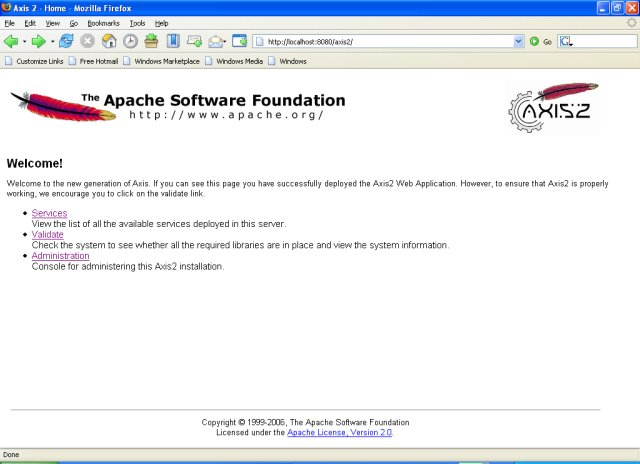
\includegraphics[scale=0.3]{../pics/axis2install.jpg}
\caption{How two different languages can deal}
\label{overflow}
\end{figure}

\end{frame}

\subsection[Short First Subsection Name]{Examples }

\begin{frame}
\frametitle{Examples}
\framesubtitle{Create a Service Class}
A StockQuoteService example seems to be mandatory in instances 
like this one, so let's use the following:
\lstinputlisting{SQS.java}
\end{frame}


\begin{frame}
\frametitle{Examples}
\framesubtitle{Generate a WSDL file from a Java class}
We need a WSDL file for our service. Axis2's 
Java2WSDL can be used to bootstrap a WSDL.
\lstinputlisting[basicstyle=\tiny]{gen.txt}
\end{frame}


\begin{frame}
\frametitle{Examples}
\framesubtitle{Structure of StockQuoteService}
The structure of this service will be as follows:
\lstinputlisting[basicstyle=\tiny]{struc.txt}
\end{frame}

\begin{frame}
\frametitle{Examples}
\framesubtitle{WSDL file of StockQuoteService}
Genereted Service Definition File:
\lstinputlisting[basicstyle=\tiny]{gened.xml}
\end{frame}


\end{document}
